\chapter{Project Specification}
Summary of the project outline.

\section{Functional Requirements}
Some text here.

\section{Non-Functional Requirements}
Some text here.

\chapter{Project Management}
Discussion on how the project was managed. What things impacted the success of the project. How does the continually revised versions of the project plan compare to the initial draft developed at the start of the project. Did everything run according to schedule. What impact did elements such as exams \& coursework have on the project. 

Undertaking a Project is a \textbf{Marathon not a Sprint}. Start immediately by firstly fully understanding what is required, start learning new languages, tools, technologies, libraries that you need and make a start on writing the report. Make full use of the time provided, making headway straight away, this will provide positive reinforcement and help propel the work along. A good analogy is that of the ``Gym'' or "DevGym" / ``Development Gym of Learning and Skills'' only by the investment of regular and consistent work, will results be achieved. As Gandalf eloquently puts it ``All we have to decide is what to do with the time that is given us'' \cite{book:Tolkien:1991:FOTR}\cite{online:Jackson:2001:FOTR}. 

Professor Randy Pausch is well known for his contribution to the ``Alice 3D'' environment as well as lectures on ``Time Management'' and ``Fulfilling your Childhood Dreams''. Both of these lectures are well worth watching, Dr. Doolan \cite{online:Doolan:2015:PauschLecture} outlines the main elements of both lectures. The post features a number of links allowing one to jump to particular segments of interest in the video lectures. Dr. Doolan \cite{online:Doolan:2016:SchwarzeneggerInterview} again highlights the key elements of success in the form of Goals, Confidence and Time Management. The post summarizes and highlights key elements of a video interview with Arnold Schwarzenegger.

\chapter{Another Appendix}

This appendix makes use of the \emph{rotating} package to rotate both figures and tables ninety degrees allowing for large datasets and illustrations to be represented.

\begin{figure}[H]
\centering
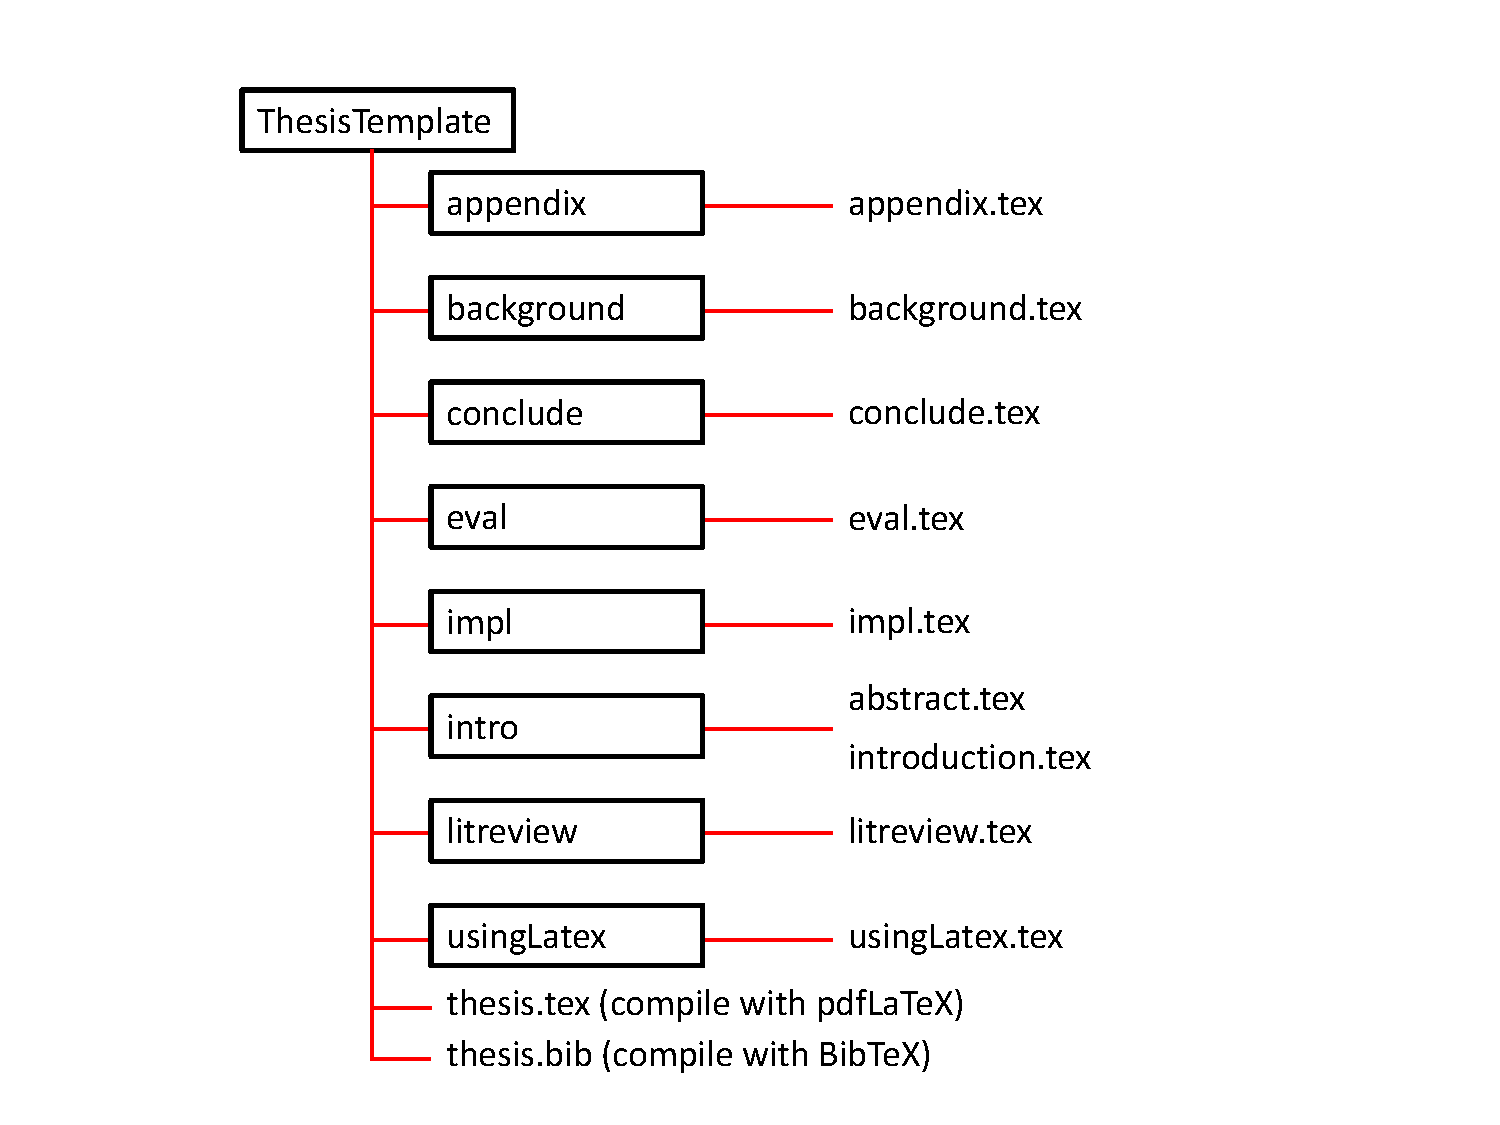
\includegraphics[width=.9\linewidth]{appendix/images/TemplateStructure.pdf}
\caption{Thesis Template Folder and \latex File Structure}
\label{fig:append:TemplateStructure}
\end{figure}

\begin{sidewaystable}
\begin{center}
   \begin{tabular}{lllllllll} 
   \toprule
   \textbf{Heading 1} & \textbf{Heading 2}  & \textbf{Heading 3}  & \textbf{Heading 4}  & \textbf{Heading 5}  & \textbf{Heading 6}  & \textbf{Heading 7}  & \textbf{Heading 8}  & \textbf{Heading 9}  \cr
   \midrule
   AAAA & BBBB & CCCC & DDDD & EEEE & FFFF & XXXX & YYYY & ZZZZ \cr 
   AAAA & BBBB & CCCC & DDDD & EEEE & FFFF & XXXX & YYYY & ZZZZ \cr 
   AAAA & BBBB & CCCC & DDDD & EEEE & FFFF & XXXX & YYYY & ZZZZ \cr 
   AAAA & BBBB & CCCC & DDDD & EEEE & FFFF & XXXX & YYYY & ZZZZ \cr 
   AAAA & BBBB & CCCC & DDDD & EEEE & FFFF & XXXX & YYYY & ZZZZ \cr 
   AAAA & BBBB & CCCC & DDDD & EEEE & FFFF & XXXX & YYYY & ZZZZ \cr 
   \bottomrule
   \end{tabular}
\caption[A Short Caption for the Table]{
	A much longer caption that will not be listed in the list of tables page.
}
\label{tab:sidewaysTable}
\end{center}
\end{sidewaystable}

\begin{sidewaysfigure}
\centerline{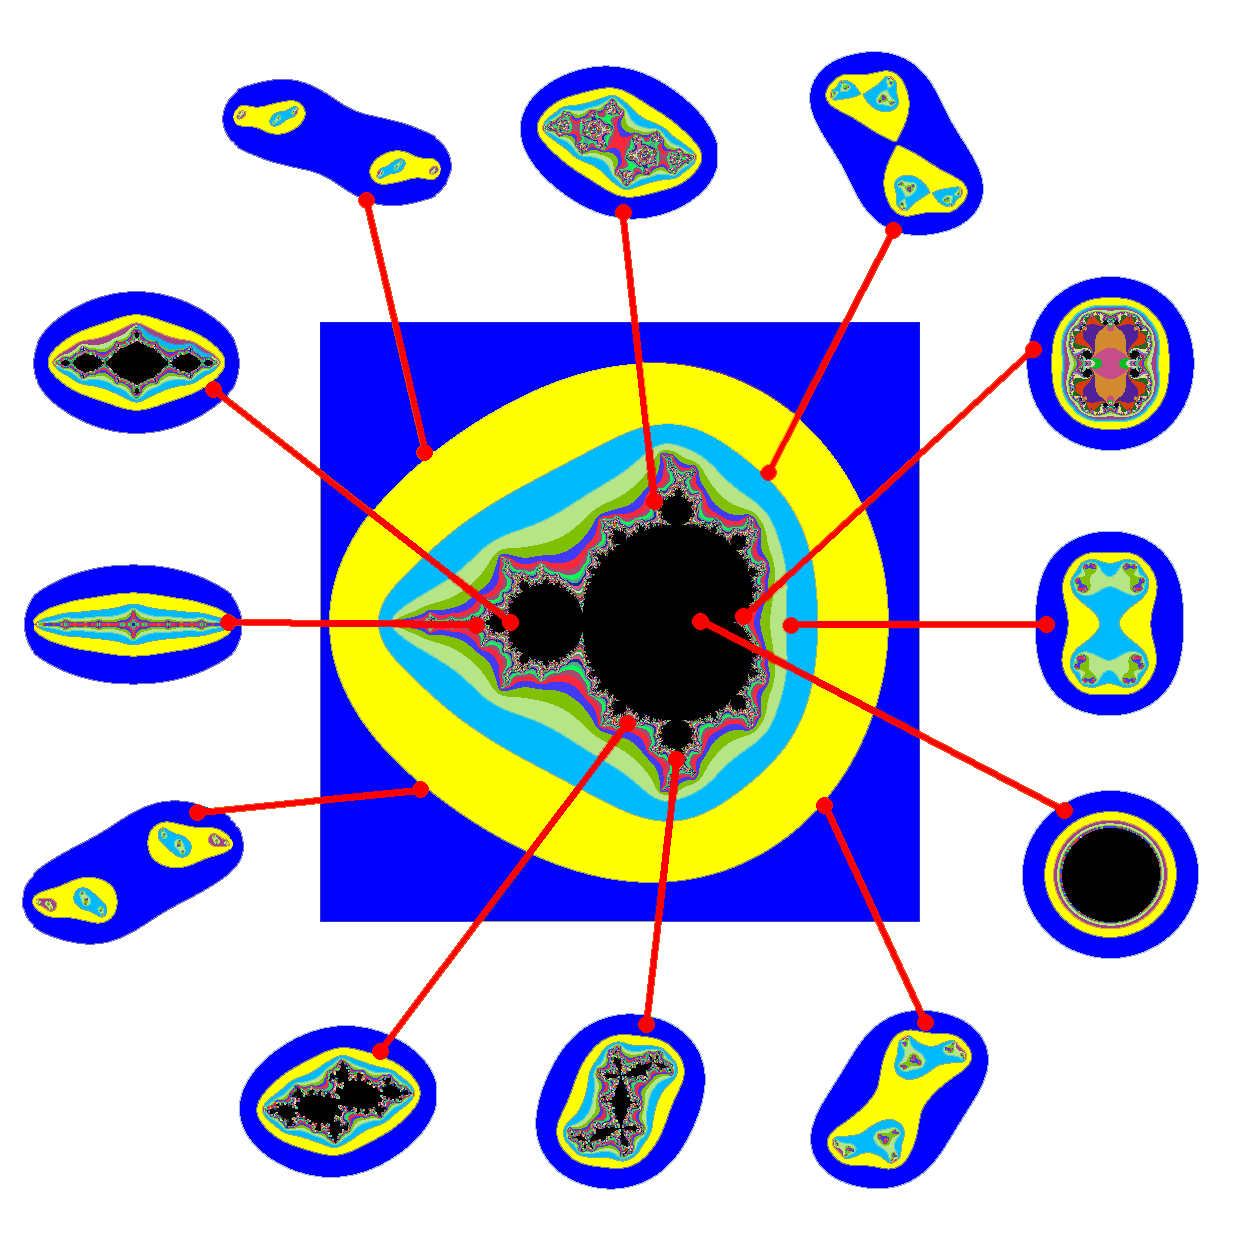
\includegraphics[width=7in]{appendix/images/samplepng}}
\caption[A Sideways Figure]{
	A much longer caption that will not be listed in the list of figures page.
}
\label{fig:sidewaysFigure}
\end{sidewaysfigure}

\chapter{Presentation Slides}
One can readily prepare presentation slides using PowerPoint or Keynote. Saving / Exporting the slides as a pdf document allows for it to be easily incorporated into this template. Each slide will be scaled to 0.45 of the \textbackslash textwidth, individual pages of the file can be accessed via the page=x option of \textbackslash includegraphics.  


\begin{figure}[H]
\parbox{74.mm}{
    \centering
    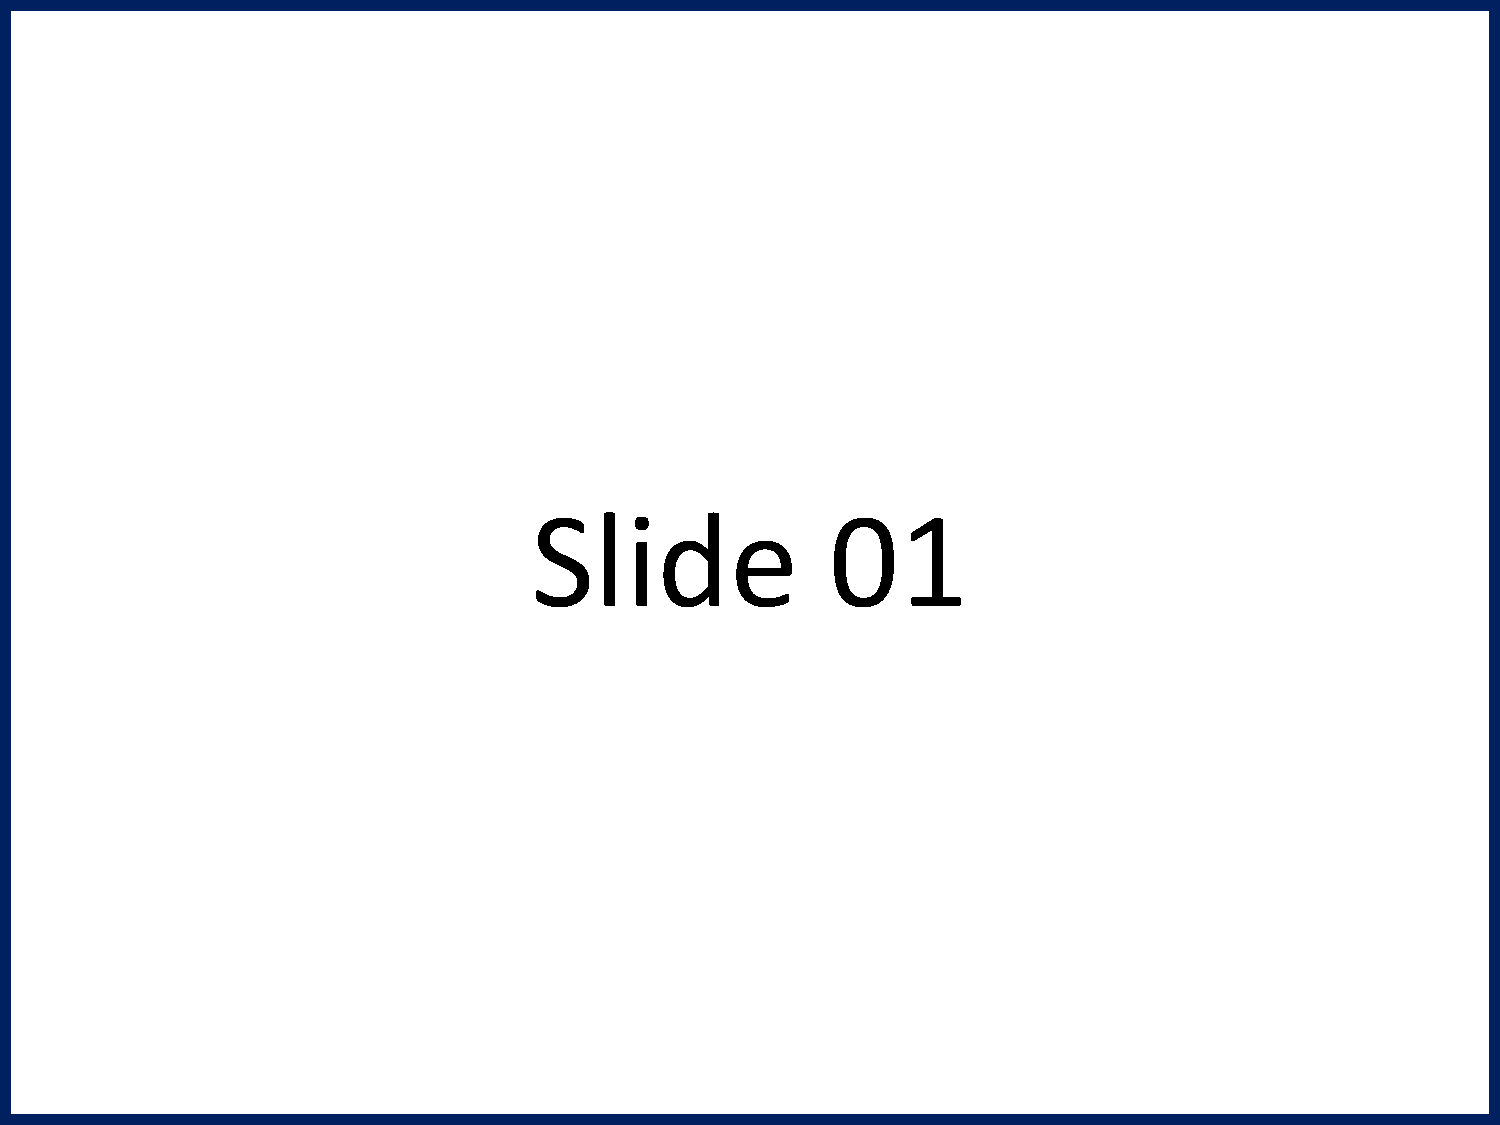
\includegraphics[width=0.45\textwidth,page=1]{appendix/images/PresentationSlides}
    \caption*{Slide 1}
}
    \parbox{74.mm}{
    \centering
    \includegraphics[width=0.45\textwidth,page=2]{appendix/images/PresentationSlides}
    \caption*{Slide 2}
}
\end{figure}

\begin{figure}[H]
\parbox{74.mm}{
    \centering
    \includegraphics[width=0.45\textwidth,page=3]{appendix/images/PresentationSlides}
    \caption*{Slide 3}
}
    \parbox{74.mm}{
    \centering
    \includegraphics[width=0.45\textwidth,page=4]{appendix/images/PresentationSlides}
    \caption*{Slide 4}
}
\end{figure}

\begin{figure}[H]
\parbox{74.mm}{
    \centering
    \includegraphics[width=0.45\textwidth,page=5]{appendix/images/PresentationSlides}
    \caption*{Slide 5}
}
    \parbox{74.mm}{
    \centering
    \includegraphics[width=0.45\textwidth,page=6]{appendix/images/PresentationSlides}
    \caption*{Slide 6}
}
\end{figure}

\begin{figure}[H]
\parbox{74.mm}{
    \centering
    \includegraphics[width=0.45\textwidth,page=7]{appendix/images/PresentationSlides}
    \caption*{Slide 7}
}
    \parbox{74.mm}{
    \centering
    \includegraphics[width=0.45\textwidth,page=8]{appendix/images/PresentationSlides}
    \caption*{Slide 8}
}
\end{figure}

\begin{figure}[H]
\parbox{74.mm}{
    \centering
    \includegraphics[width=0.45\textwidth,page=9]{appendix/images/PresentationSlides}
    \caption*{Slide 9}
}
    \parbox{74.mm}{
    \centering
    \includegraphics[width=0.45\textwidth,page=10]{appendix/images/PresentationSlides}
    \caption*{Slide 10}
}
\end{figure}

\chapter{Project Log}

The following is a weekly summary of the work carried during the development of this body of work. It covers tasks that were completed, tutorials that were worked through, articles that were read and summaries of discussions / meetings held with the project supervisor and other third parties. 

\section*{Week Beginning: Monday 26/09/2022}

First week working on the project. Had a meeting with supervisor and discussed some of the issues related to the project. The first deliverable is due for the end of next week (project outline \& ethics form). 

\begin{itemize}
  \item Downloaded and Installed \latex (MikTeX full install) and TeXmaker. 
  \item Started to get to grips with the \latex system by making simple modifications to the template and editing the project log.
  \item Developed a Mind Map to clarify understanding of project elements.
  \item Prepared an initial draft of project plan in the form of a Gantt chart. 
  \item Prepared and revised draft of project proposal. 
  \item Downloaded and read half a dozen BSc \& MSc Project Reports to see the general format and expected content. A list of the reports could be included here.
  \item Started learning how to use some API's needed for the project. 
  \item Looked on the University Library website for link to the ``Databases'' area providing access to repositories such as IEEE Explore and ACM Digital Library. 
\end{itemize}



